\subsection{Asynchronous and Parallel Compilation}
\label{sec:framework}
The need for fast generation of specialized circuits is mostly explained by the the known computer science laws being challegend (dennard, moore, the walls, dark silicon era).
A recent and emerging solution that allows to follow the pace is OpenSource EDA and its community~\cite{Openroad}.
We adopt this approach and build our own open source tool.
Figure~\ref{fig:suf} depicts this framework which enables the generation of many independant design entries from high level description in python to silicon GDS.

\begin{figure}[t]
\centering
	\vspace{-0.5cm}
	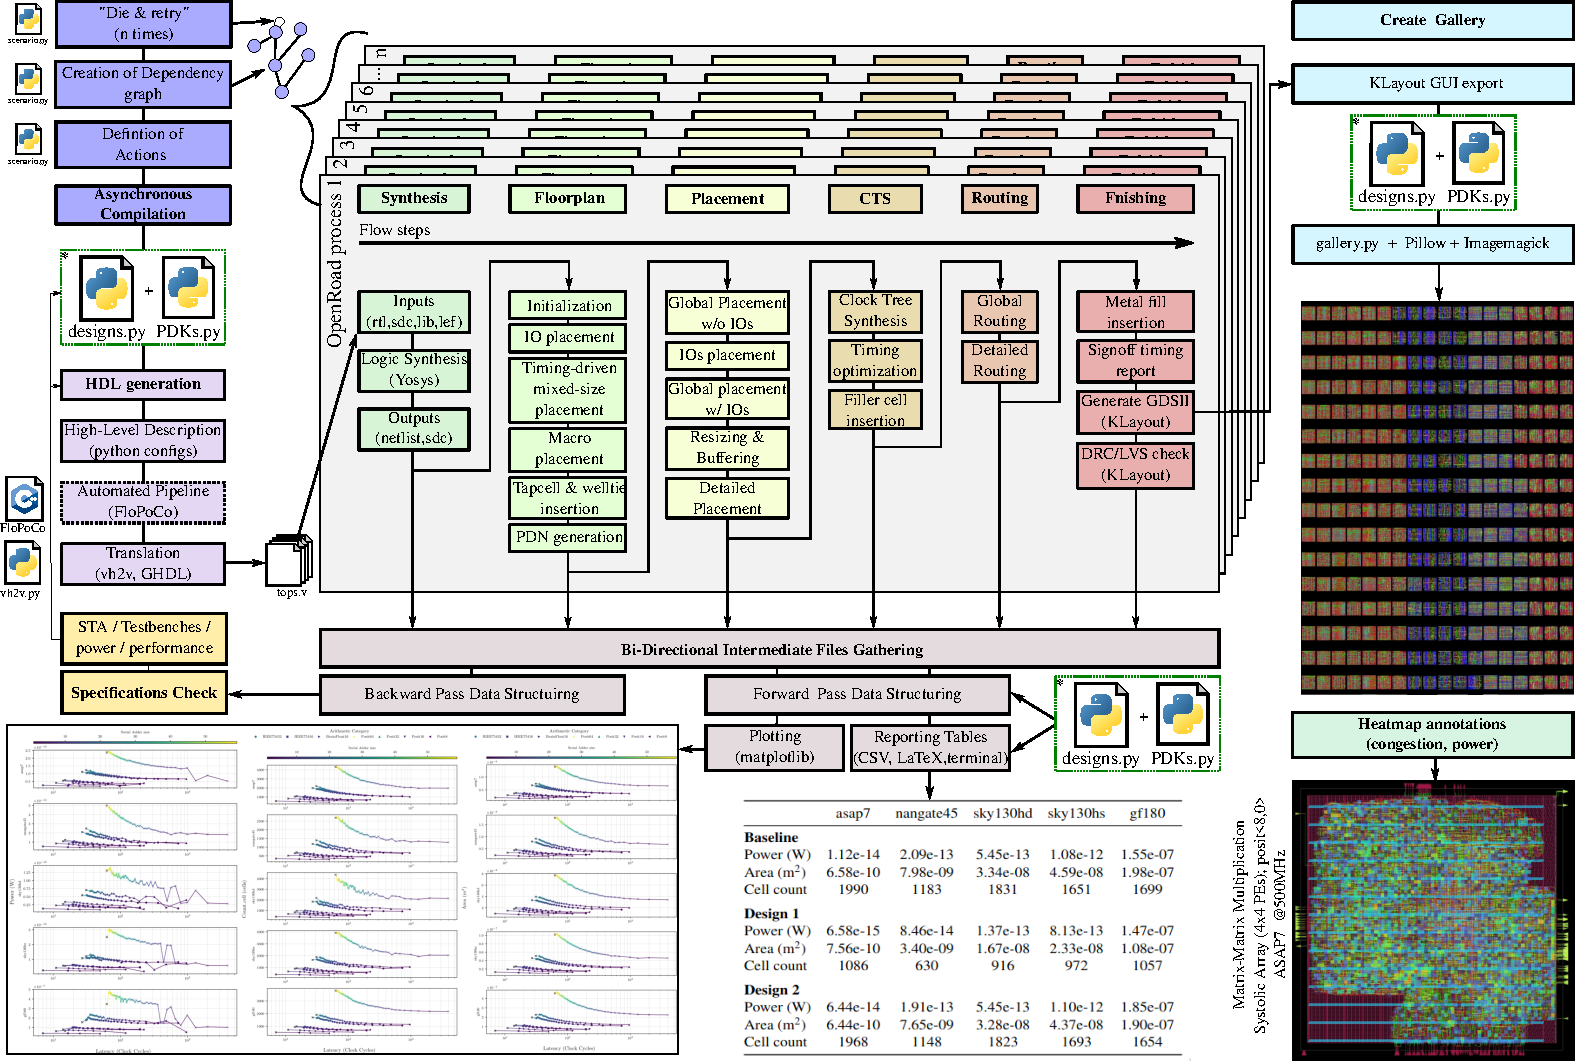
\includegraphics[width=\columnwidth]{./figures/SUF.pdf}
	\vspace{-0.5cm}
	\caption{Schematic Overview SUF: Centralized Management of Asynchronous OpenROAD Forks, Derived from Dependency Task Graphs. This illustration also encapsulates the extended capabilities ranging from Code Generation without manual RTL Writing to Advanced Plotting and Visualization Features.}
	\label{fig:suf}
\end{figure}

\begin{figure}[b]
\centering
	\vspace{-0.5cm}
	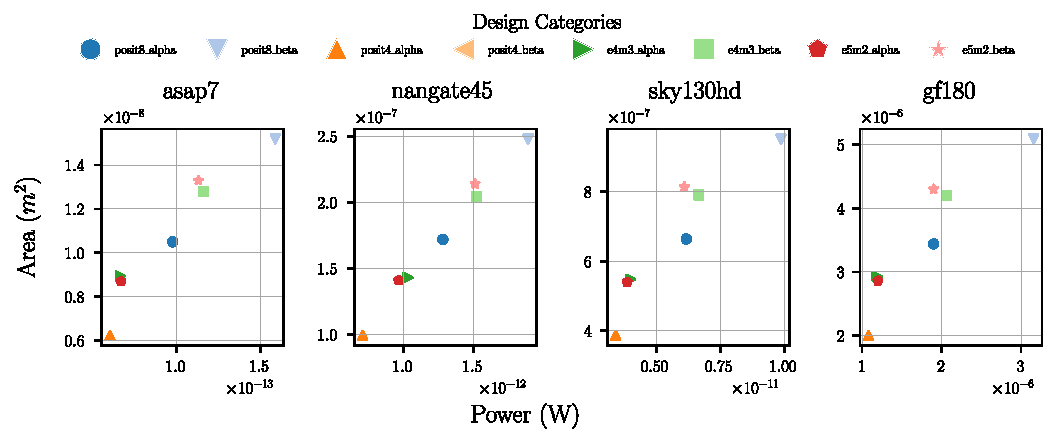
\includegraphics[width=\columnwidth]{./figures/power_vs_area_comparison.pdf}
	\vspace{-0.5cm}
	\caption{Area vs. Power}
	\label{fig:power_vs_area}
\end{figure}

\subsection{Functional and Performance Specifications}
\label{sec:specifications}
We define and assess four computational formats distinguished by their compactness and mathematical attributes (dynamic range).
These include Nvidia's e4m3 and e5m2, and the tapered formats, posit4 (es=0), and posit8(es=2)~\cite{}.
Another significant aspect of our work is the proposal of two variations of internal paths for each of these formats.
Internally, we execute the dot product as a fused operation (without rounding) in a fixed accumulator with varying boundaries (bit weights for lsb/msb/ovf).
These variations, named $\alpha$ and $\beta$, are configured as follows: $(\text{ovf}=2,\text{msb}=3,\text{lsb}=-2)$ for an aggregate of 8 bits, and $(\text{ovf}=5,\text{msb}=5,\text{lsb}=-5)$ for the 16-bit model.
The weights distribution of the embedding layers in the Llama-2-7b model~\cite{} dictates these boundaries.
%It is vital to evaluate the trade-offs in the accelerator segment robustly, considering the dynamic range of formats, precision, and sequentialism inherent in MMM algorithms.
All Systolic Arrays of this work are set to $8x8=64$ PEs, which ends the defintion of the \textit{Functional} specifications set.

% Performance properties
We complement this set with \textit{Performance} specifications that span four accross four PDKs, namely GF180, Sky130hd, nangate45, and ASAP7 which are all open (TBD).
Evaluation of several PDKs allow to verify scalability of designs without the use of manual scaling which are often (make it formal and scientific).

\subsection{Results}
The evaluation of 14 design entries, with posit 4 beta not working finished in two hours yielding a total of xx chips.
Figure~\ref{fig:power_vs_area} shows depicts power and area accross 5 process nodes.



\begin{figure}[t]
\centering
	\vspace{-0.5cm}
	\includegraphics[width=0.5\columnwidth]{./figures/SA_8x8_e4m3_rulers_congestion.png}
	\vspace{-0.5cm}
	\caption{e4m3 cogestion routed highlighted beta 8x8}
	\label{fig:focus on e4m3}
\end{figure}

\begin{figure}[t]
\centering
	\vspace{-0.5cm}
	\includegraphics[width=\columnwidth]{./figures/systolic_arrays.png}
	\vspace{-0.5cm}
	\caption{All generated arrays}
	\label{fig:all_arrays}
\end{figure}

